% !TeX root = ../thesis.tex

\chapter{Experiments and Evaluation}
\label{sec:experiment_evaluation}

In this chapter, we first make a brief introduction to the hardware development platform and the datasets employed in our pipeline. Then we conduct three experiements both on groudtruth and original videos to evaluate the effectiveness and run-time performance of our pipeline. At last the experiment results will be discussed. 

\section{Hardware Platform}

During the development of our pipeline, we mainly employ two types of hardware platform: Nvidia Jetson TX2 Developer Kit\footnote{\url{https://elinux.org/Jetson_TX2}} for pipeline development and Server equipped with GeForce GTX 1080 GPUs\footnote{\url{https://www.nvidia.com/en-us/geforce/products/10series/geforce-gtx-1080/}} for real-time testing.

\textbf{Nvidia Jetson TX2 Developer Kit}

NVIDIA Jetson TX2 is an embedded system-on-module (SoM) with dual-core NVIDIA Denver2 + quad-core ARM Cortex-A57, 8GB 128-bit LPDDR4 and integrated 256-core Pascal GPU. Its board and module components are shown in Figure \ref{fig:tx2_board} and \ref{fig:tx2_module}. 

\begin{figure}[h!]
  \centering
  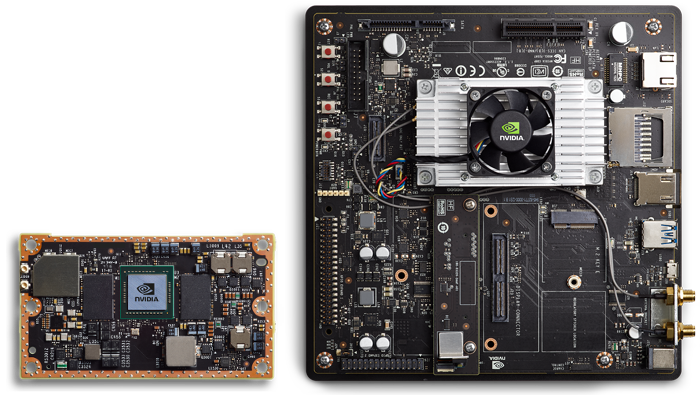
\includegraphics[width=0.6\linewidth]{ExpAndDiss/tx2_board.png}
  \caption{Nvidia Jetson TX2 Board}
  \label{fig:tx2_board}
\end{figure} 

\begin{figure}[h!]
  \centering
  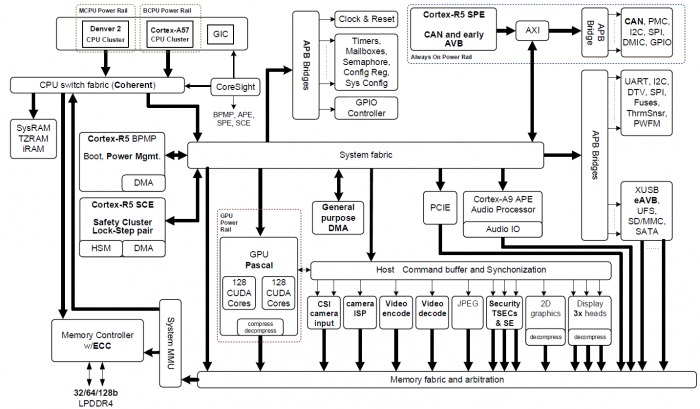
\includegraphics[width=0.6\linewidth]{ExpAndDiss/tx2_module.png}
  \caption{Nvidia Jetson TX2 Module Diagram}
  \label{fig:tx2_module}
\end{figure} 


\section{Datasets}
In our pipeline, we mainly work on the dataset Joint Attention in Autonomous Driving (JAAD) \cite{DBLP:journals/corr/KotserubaRT16}. 

\subsubsection{JAAD Dataset}

As presented in \cite{rasouli2017they}, JAAD dataset is a new dataset for studying joint attention in the context of autonomous driving. In particular, the focus is on pedestrian and driver behaviors at the point of crossing and factors that influence them. To this end, JAAD dataset provides an annotated collection of short video clips representing scenes typical for everyday urban driving in various weather conditions.

JAAD dataset contains 346 high-resolution video clips (most are 5-10 sec) extracted from approximately 240 hours of driving videos filmed in several locations in North America (60 clips) and Eastern Europe (286 clips) using three different high-resolution monocular cameras with a frame rate of 30 fps. The dataset comes with three types of ground truth annotations: bounding boxes for
detection and tracking of pedestrians, behavioral tags indicating the state of the pedestrians and scene annotations listing the environmental contextual elements. 

\textbf{Bounding boxes}

the dataset contains approximately 82k frames and 2.2k unique pedestrian samples comprising a total of 337k bounding boxes. Occlusion information is provided in the form of tags for each bounding box: partial occlusion (between 25 and 75\% visible) and full occlusion (less than 25\% visible). $\sim$55K (13\%) of bounding boxes are tagged with partial occlusion and $\sim$49K (12\%) with heavy occlusion.

\textbf{Behavioral tags}

Behavioral data and attributes are provided for 868 pedestrians. Figure \ref{fig:jaad_bahavior_label} illustrates a scene of a temporal behavioral labels in the dataset.

\begin{figure}[h!]
  \centering
  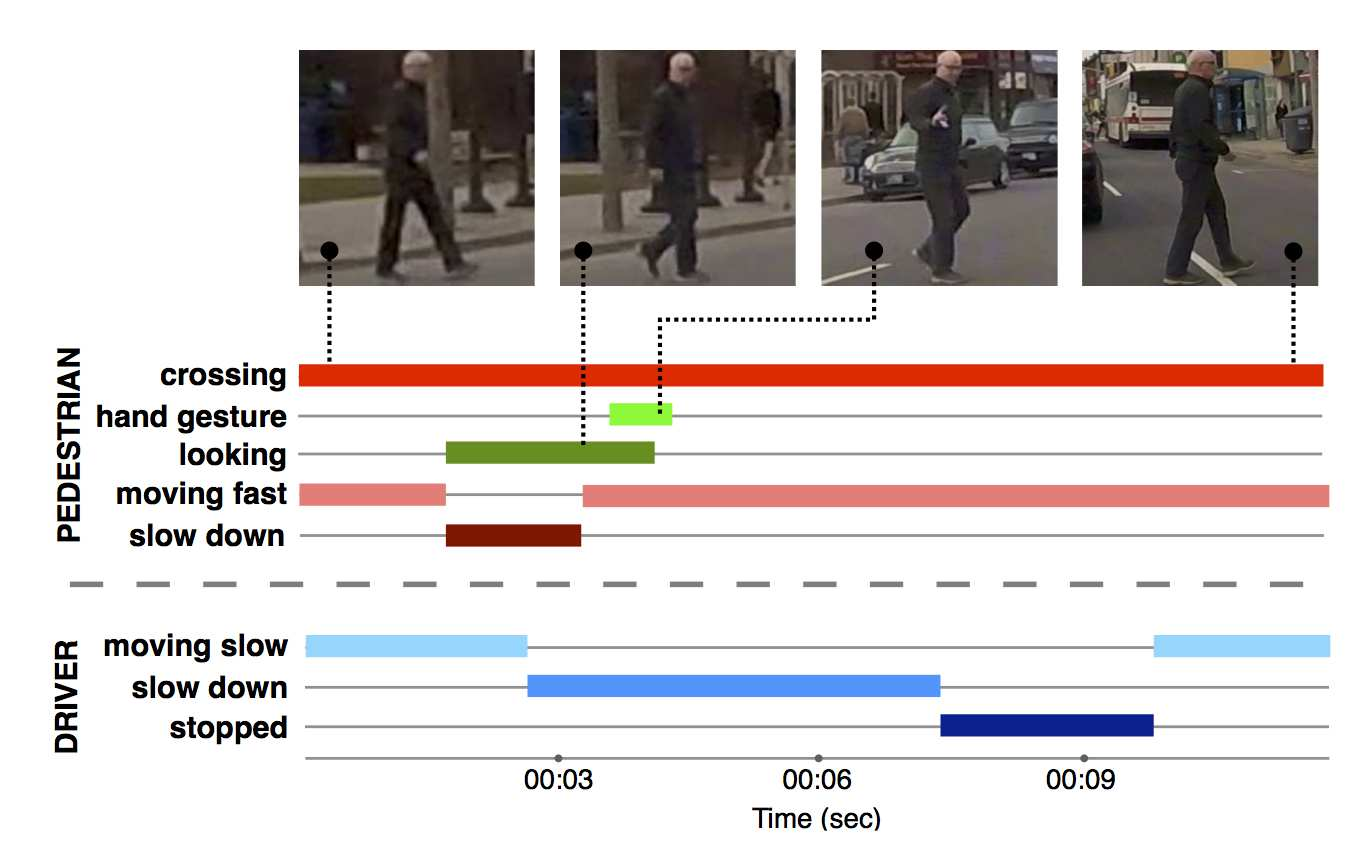
\includegraphics[width=0.6\linewidth]{ExpAndDiss/jaad_behavior_label.png}
  \caption{Behavioral labels with timestamps to represent the sequence of the events that took place during the crossing and observe
           the correspondence between the actions of the driver and the pedestrian. \cite{rasouli2017they}}
  \label{fig:jaad_bahavior_label}
\end{figure}

The pedestrians’ actions are categorized into 3 groups: 

\begin{description}[leftmargin=0in, labelindent=0pt]
\item[Precondition] this refers to the state of the pedestrian prior to crossing and can be either standing, moving slow or fast.

\item[Attention] the way the pedestrian becomes aware of the approaching vehicle. These actions, depending on their duration, are looking (> 1s) or glancing ($\leq$ 1s).

\item[Response] this includes the behaviors that pedestrians exhibit in response to the action of the approaching vehicle, namely, stop, clear path, slow down, speed up, hand gesture and nod. 
\end{description}

\textbf{Contextual tags}

Each frame is assigned a contextual tag that describes the scene. There are four types of contextual information: 

\begin{description}[leftmargin=0in, labelindent=0pt]
\item[Configuration] includes the number of lanes or whether it is a parking lot/garage.

\item[Traffic signals] refers to the presence of zebra crossing, pedestrian sign, stop sign or traffic light in the scene.

\item[Weather] includes sunny, cloudy, snowy or rainy.

\item[Time of day] this tag crudely indicates the lighting conditions and can be day, afternoon or nighttime.
\end{description}

Figure \ref{fig:jaad_pedestrian_samples} displays some selected pedestrians from the dataset.

\begin{figure}[h!]
  \centering
  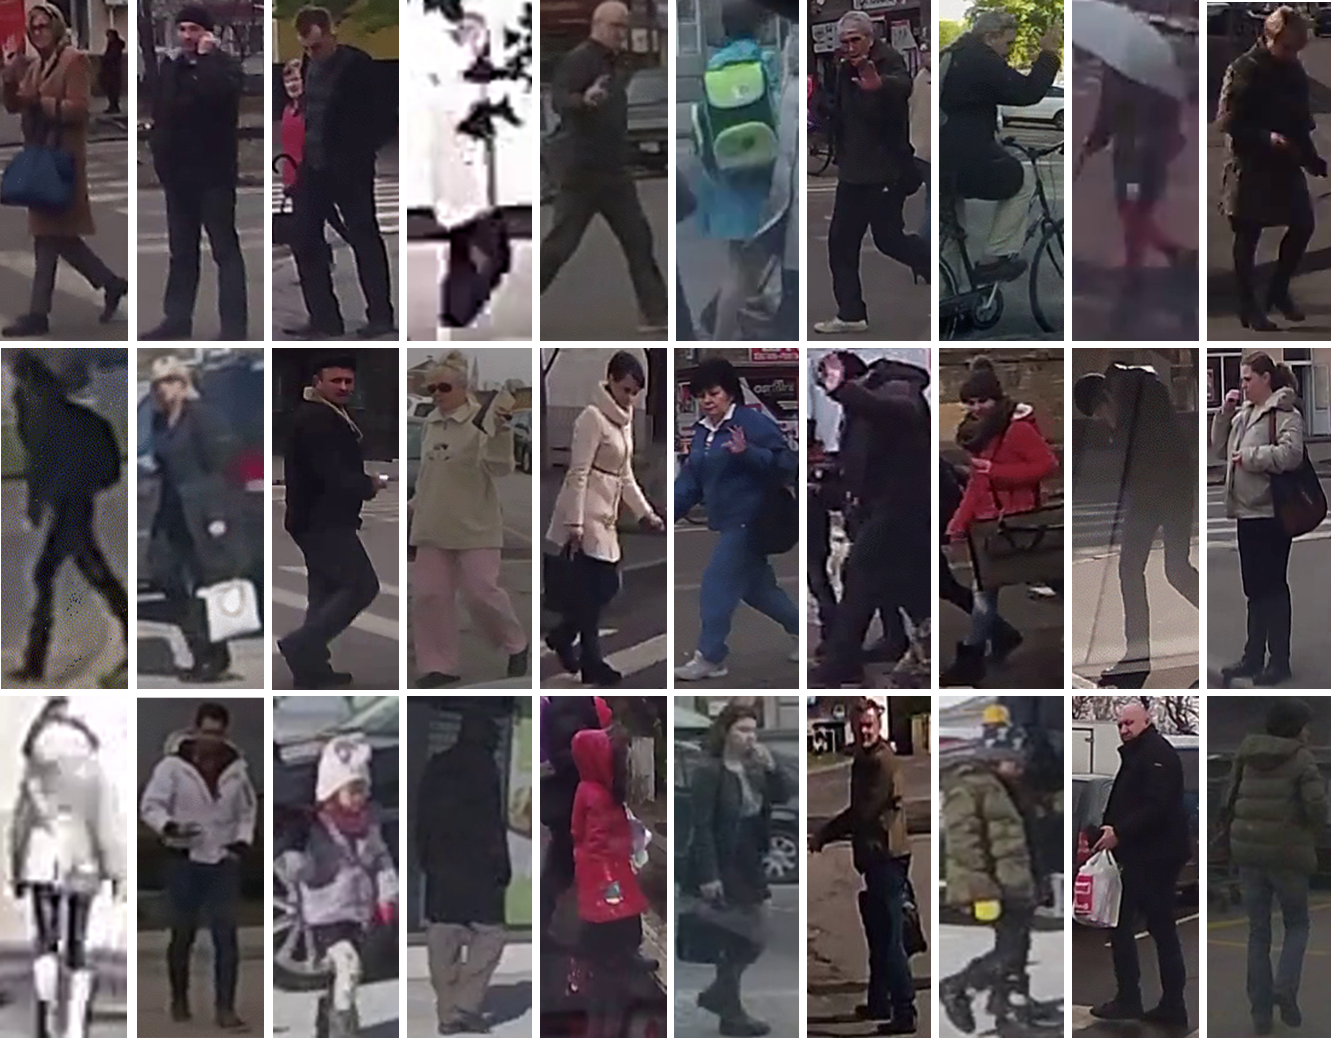
\includegraphics[width=0.6\linewidth]{ExpAndDiss/jaad_pedestrian_samples.png}
  \caption{A selection of images of pedestrians from the dataset. \cite{rasouli2017they}}
  \label{fig:jaad_pedestrian_samples}
\end{figure}

\section{Experiments}
The experiments pipeline is as follows, shown in Figure \ref{fig:exp_pipe}:

\begin{figure}[H]
  \centering
  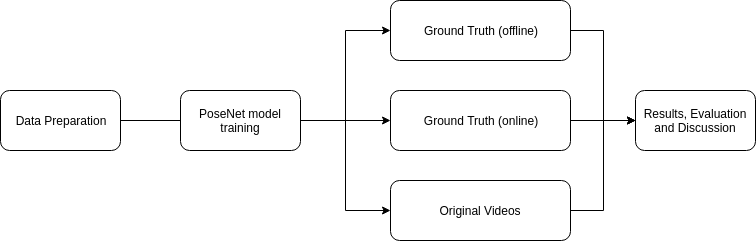
\includegraphics[width=0.8\linewidth]{ExpAndDiss/exp_pipe.png}
  \caption{The pipeline of experiments}
  \label{fig:exp_pipe}
\end{figure}

\textbf{Data Preparation}

The training of PoseNet is based on the ground truth from JAAD dataset, which contains image sequences of 698 pedestrians from different video clips. For each pedestrian image sequences, we first extract 3D pose of each frame and write the data in Hierarchical Data Format\footnote{\url{https://en.wikipedia.org/wiki/Hierarchical_Data_Format}} (HDF5). As introduced above, we traverse the body map to form the pose tensor, in our experiments, we set the traversal sequence to [6, 2, 1, 0, 1, 2, 6, 3, 4, 5, 4, 3, 6, 8, 9, 8, 12, 11, 10, 11, 12, 8, 13, 14, 15, 14, 13, 8, 6], which stands for ['Pelvis', 'RHip', 'RKnee', 'RAnkle', 'RKnee', 'RHip', 'Pelvis', 'LHip', 'LKnee', 'LAnkle', 'LKnee', 'LHip', 'Pelvis', 'Neck', 'Head', 'Neck', 'RShoulder', 'RElbow', 'RWrist', 'RElbow', 'RShoulder',  'Neck', 'LShoulder', 'LElbow', 'LWrist', 'LElbow', 'LShoulder', 'Neck', 'Pelvis'] in the model topology shown in Figure \ref{fig:pose_topo}. Then we get 698 h5 files, each of them contains the pose keypoints of a pedestrian with the shape of (N, M), here N is the number of frames and M stands for the number of joint positions, which, in our case, is 87 (= 29 $\times$ 3, 29 is the number of traversal sequence nodes listed above, 3 stands for $(x, y, z)$). 

\textbf{PoseNet Model Training}

At the stage of training, we utilize the PoseNet model as described here in Figure \ref{fig:posenet_3d} and generate pose tensor of 10 frames. Here we train several models, one is trained exactly the way the pipeline works, which is generating pose tensor at each frame (expect for the first 10 frames), one is trained with data jittering augmentation, which is supposed to compensate the negative effects brought by the rapid change of camera perspective and instability of bounding box obtained from \textit{Person Tracker} and another one is trained with random strides of pose tensor. 

\textbf{Implementation}

\begin{itemize}
\item[•] \textbf{Ground Truth (offline)}

The first experiment we conduct after training PoseNet model is to apply them on the h5 files to validate the effectiveness of data processing together with the action grouping strategy in the pipeline. What we do is to read the pose keypoints from the h5 files and store them in numpy arrays. Then we generate pose tensor the way the pipeline works. At last we write the final action labels to file and group the same action category with the corresponding frame ID. Since in our baseline, we have the start and end frames of an action performed by a single pedestrian in one video clip, so we arrange the action classification results into the same pattern, i.e. [start\_frame, end\_frame, action]. After that, we take the IoU between our experiments result and the baseline as the evaluation metrics, which is illustrated in Figure \ref{fig:iou_case}.

\begin{figure}[H]
  \centering
  \subfigure[Example case 1]{
  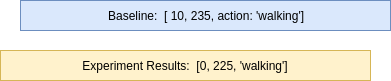
\includegraphics[width=0.5\linewidth]{ExpAndDiss/case_1.png}}  
  \subfigure[Example case 2]{
  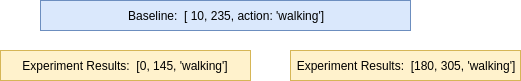
\includegraphics[width=0.6\linewidth]{ExpAndDiss/case_2.png}}
  \caption{Example cases for IoU between baseline and expriment results. In case 1, the Union of two results is the frame range [0,
           235], and the Intersection is [10, 225], then the IoU = Intersection / Union, which is (225 - 10 + 1) / (235 - 0 + 1) =
           91.5\%. While in case 2, the Union is [0, 305], and the Intersection is [10, 145] $\cup$ [180, 235], so the IoU is ((145
           - 10 + 1) + (235 - 180 + 1)) / (305 - 0 + 1) = 62.7\%}
  \label{fig:iou_case}
\end{figure} 

\item[•] \textbf{Ground Truth (online)}

The second experiments we plan is to feed the image sequences as input to the pipeline, tring to get a primary conclusion if the detection, tracking as well as pose estimation part together work reasonably. We also make the comparion of the results between this experiment and the baseline just like the offline testing occasion.

\item[•] \textbf{Original Videos}

After running testing on ground truth, we now run the pipeline on the original videos in the JAAD dataset. Unlike the ground truth, the original videos contains many more agents, a quantitive comparison between the runtime results and baseline is impossible. One possible scenario is shown in Figure \ref{fig:runtime_demo}. 

\begin{figure}[h!]
  \centering
  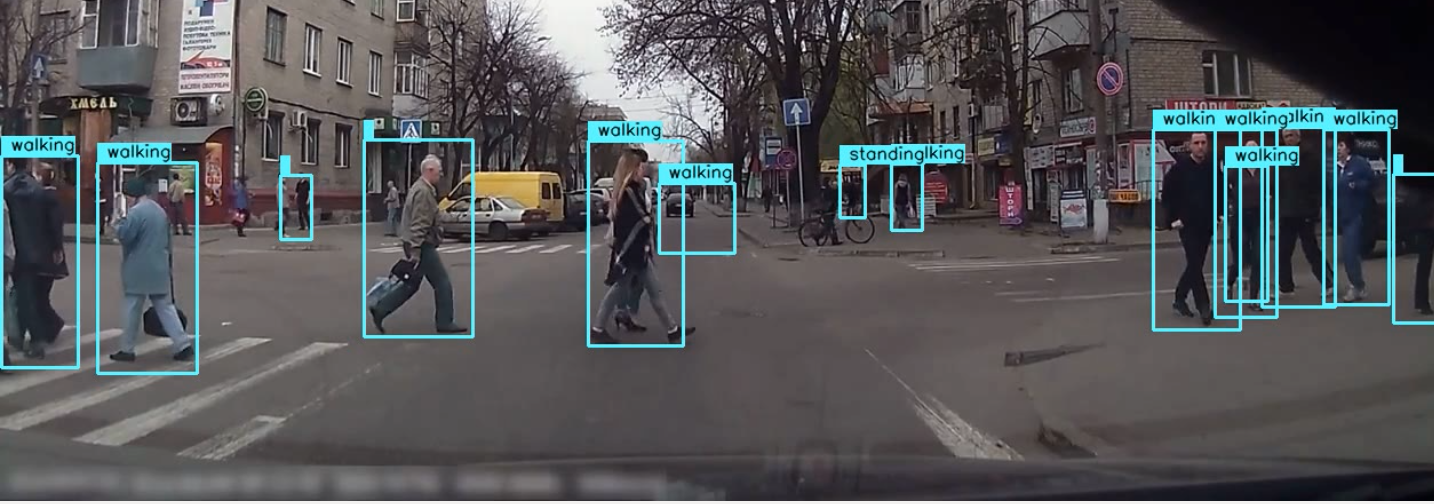
\includegraphics[width=0.9\linewidth]{ExpAndDiss/runtime_demo.png}
  \caption{The pipeline of experiments}
  \label{fig:runtime_demo}
\end{figure}

\end{itemize}


\section{Results and Discussion}
\label{sec:eval}

In this section we will present the results of the experiments, and evaluate the performance on the metrics of IoU (\%), frame rate (fps) as well as latency (ms) between ROS nodes. 

\textbf{Results}

In the experiments, we set two main variables: PoseNet model, testing fashion. We also suppose that only the pedestrians with a IoU of at least 0.5 are successfully processed, as our pipeline only classifies two categories (walking or standing), theoretically a random posibility of either action would be 0.5. Table \ref{tab:iou_result} shows the result of experiments 1 and 2.

\begin{table}[H]
\centering
\caption{Experiment results: ground truth offline and online testing}
\begin{tabular}{lll}
\hline                                                                                                      &  & \multicolumn{1}{c}{\textbf{IoU}}                                                                          \\ \hline
\multicolumn{1}{c}{\begin{tabular}[c]{@{}c@{}}Ground Truth (offline) \\  jittering model\end{tabular}} &  & \multicolumn{1}{c}{\begin{tabular}[c]{@{}c@{}}0.902\\ Total videos: 698, valid videos: 636\end{tabular}}  \\
                                                                                                       &  &                                                                                                           \\
\multicolumn{1}{c}{\begin{tabular}[c]{@{}c@{}}Grund Truth (offline) \\ stride 1 model\end{tabular}}    &  & \multicolumn{1}{c}{\begin{tabular}[c]{@{}c@{}}0.921\\ Total videos: 698, valid videos: 640\end{tabular}}  \\
                                                                                                       &  &                                                                                                           \\
\multicolumn{1}{c}{\begin{tabular}[c]{@{}c@{}}Ground Truth (online)\\  jittering model\end{tabular}}   &  & \multicolumn{1}{c}{\begin{tabular}[c]{@{}c@{}}0.716\\ Total videos: 676,  valid videos: 337\end{tabular}} \\
                                                                                                       &  &                                                                                                           \\
\multicolumn{1}{c}{\begin{tabular}[c]{@{}c@{}}Ground Truth (online)\\  stride 1 model\end{tabular}}    &  & \multicolumn{1}{c} 
{\begin{tabular}[c]{@{}c@{}}0.697\\ Total videos: 676,  valid videos: 339\end{tabular}} \\ 
\hline
\end{tabular}
\label{tab:iou_result}
\end{table}

As our pipeline is aimed to be running in real-time, we have made a run-time performance testing both on Nvidia Jetson TX2 and GPU Server. The testing is running on the JAAD original videos, and the frame rate of each node in the pipeline is evaluated, as shown in Table \ref{tab:runtime_performace}.

\begin{table}[h!]
\centering
\caption{Run-time performance of each node in the pipeline}
\begin{tabular}{cllc}
\hline
\textbf{ROS node}    &  &  & \textbf{FPS}                                                                                        \\ \hline
/person\_detector    &  &  & \begin{tabular}[c]{@{}c@{}}Nvidia Jetson TX2:  2 $\sim$3 \\ GPU Server:  35 $\sim$40\end{tabular}   \\
\multicolumn{1}{l}{} &  &  & \multicolumn{1}{l}{}                                                                                \\
/person\_tracker     &  &  & \begin{tabular}[c]{@{}c@{}}Nvidia Jetson TX2:  3 $\sim$5 \\ GPU Server:  4 $\sim$5\end{tabular}     \\
\multicolumn{1}{l}{} &  &  & \multicolumn{1}{l}{}                                                                                \\
/pose\_3d\_ros       &  &  & \begin{tabular}[c]{@{}c@{}}Nvidia Jetson TX2:  3 $\sim$5 \\ GPU Server:  10 $\sim$15\end{tabular}   \\
\multicolumn{1}{l}{} &  &  & \multicolumn{1}{l}{}                                                                                \\
/data\_manager\_3d   &  &  & \begin{tabular}[c]{@{}c@{}}Nvidia Jetson TX2:  30 $\sim$40 \\ GPU Server:  $\sim$100\end{tabular}   \\
\multicolumn{1}{l}{} &  &  & \multicolumn{1}{l}{}                                                                                \\
/pose\_net\_3d       &  &  & \begin{tabular}[c]{@{}c@{}}Nvidia Jetson TX2:  15 $\sim$20 \\ GPU Server:  40 $\sim$50\end{tabular} \\
\multicolumn{1}{l}{} &  &  & \multicolumn{1}{l}{}                                                                                \\
/visual\_agency      &  &  & \begin{tabular}[c]{@{}c@{}}Nvidia Jetson TX2:  20 $\sim$30 \\ GPU Server:  $\sim$50\end{tabular}    \\ \hline
\end{tabular}
\label{tab:runtime_performace}
\end{table}

\textbf{Discussion}

As we can see from Table \ref{tab:iou_result}, the offline ground truth testing results in a very high alignment with baseline. Here jittering model doesn't have a better performance than the other model, as offline pose data dosen't change on the running. From these results, we could verify that the data processing is also valid during run-time. While for the online testing on ground truth, the IoU shows an obviously lower value, and almost half of the videos are invalid. There exist some possible explanations. 

\begin{itemize}
\item[•] \textbf{Detection and tracking failure} 

As mentioned in Section \ref{pipeline:PD} and \ref{pipeline:PT}, the person detector and person tracker can not fit in all scenarios with the same parameters settings. After some exploration, we find that the size of the person bounding box plays an important role here. As our PoseNet models are trained on the ground truth from JAAD dataset, the pedestrians are always at the center of the image and almost occupy the whole area of the image frames. While in run-time situation, the bounding box obtained from tracking always change, and the person image, which will then be padded and   


\end{itemize}   









%\sisetup{round-mode = places, round-precision = 2, scientific-notation = fixed, fixed-exponent = 0}
%\begin{table}[h!]%[!htbp]
%    \centering
%    \begin{tabular}{crSSSSSS}
%        \hline
%        & & \textbf{mean} & \textbf{median} & \textbf{stddev} & \textbf{min} & \textbf{max} & \textbf{other}\\%
%        \hline
%        \parbox[t]{2mm}{\multirow{3}{*}{\rotatebox[origin=c]{90}{Data1}}}
%        & Lane 1 [m] & 3.78e+00 & 3.78e+00 & 8.06e-02 & 3.58e+00 & 4.23e+00 & 3.75\\
%        & Lane 2 [m] & 3.84e+00 & 3.84e+00 & 4.58e-02 & 3.58e+00 & 4.02e+00 & 3.75\\
%        & Lane 3 [m] & 3.82e+00 & 3.81e+00 & 8.30e-02 & 3.31e+00 & 4.06e+00 & 3.75\\
%        \hline
%    \end{tabular}
%    \caption[Short Description for List of Tables]{
%      Long Description for under the table.
%    }\label{tab:xy}
%\end{table}

% results table (fps, latency, accuracy/effectiveness) [frame n -> frame m, label]
% ros related: nodelet, (c++ vs python)
% validation of person detection and person tracking => detection vs tracking 
% sensitive tracking bbox --> training not pose normalization






